\documentclass{article}
\usepackage[utf8]{inputenc}
\usepackage[T1]{fontenc}
\usepackage[english]{babel}
\usepackage{graphicx}
\usepackage{physics}
\usepackage{calrsfs}
\usepackage{mathalpha}
\usepackage{amssymb}
\usepackage{amsfonts}
\usepackage{amsmath}
\usepackage{fixltx2e}
\usepackage{enumitem}
\usepackage{float}
\usepackage[table]{xcolor}
\newcommand*\xor{\mathbin{\oplus}}
\usepackage{xcolor}
\usepackage{braket}
\usepackage{tikz}
\usepackage{hyperref}
\hypersetup{
  colorlinks=true,
  linkcolor=blue
}

\renewcommand{\labelitemi}{-}
\renewcommand{\labelitemii}{+}

\usepackage[dvipsnames]{xcolor}

\definecolor{myDarkGreen}{RGB}{0, 128, 0}

\title{Lesson 2021-04-27 (Week 8)}
\begin{document}
\date{}
\maketitle
\author{}
\date{}

\maketitle
\section{Bit commitment (recall)}
Let's examine what is a commitment in cryptography by using this example: \newline 
Stockbroker Alice wants to convince investor Bob that her method of picking winning stocks is sound.


\begin{itemize}
    \item \textbf{Bob}: “Pick five stocks for me. If they are all winners, I’ll give you my business.”
    \item \textbf{Alice}: “If I pick five stocks for you, you could invest in them
without paying me. Why don’t I show you the stocks I picked last
month?”
\item \textbf{Bob}: “How do I know you didn’t change last month’s picks after
you knew their outcome? If you tell me your picks now, I’ll know
that you can’t change them. I won’t invest in those stocks until
after I’ve purchased your method. Trust me.”
\item \textbf{Alice}: “I’d rather show you my picks from last month. I didn’t
change them. Trust me.”
\end{itemize}

From a cryptographical point of view, basically Alice wants to commit to a prediction (i.e., a bit or series of bits) but does not
want to reveal her prediction until sometime later. Bob, on the other hand, wants to make sure that Alice cannot change her mind after she has committed to her prediction.
In general a commitment scheme is a protocol for Alice and Bob with two different phases and one algorithm \textit{Com}:
\begin{enumerate}
\item \textbf{"Commitment phase"}: Alice has a secret $b$ to commit and sends to Bob the commitment value $c$ (commitment for b). The value $c$ is the output $c=Com(b, r)$ of the algorithm $Com$. $r$ indicates that $c$ is computed by $b$ and some random value $r$.
\item \textbf{"Opening/reveal phase"}: Alice sends to Bob the former secret $b$, then Bob can check $c=Com(b,r)$ for $r$.
\end{enumerate}
A possible implementation of this protocol uses symmetric cryptography:
\begin{enumerate}
    \item Bob generates a random-bit string, R, and sends it to Alice.
    \item Alice creates a message consisting of the bit she wishes to commit to, $b$ (it can actually be several bits), and Bob’s random string. She encrypts it with some random key, $K$, and sends the result back to Bob \rightarrow $Enc_K(R,b)$ (The Encryption algorithm is actually the previous $Com$). That is the commitment portion of the protocol. Bob cannot decrypt the
message, so he does not know what the bit is.
When it comes time for Alice to reveal her bit, the protocol continues:
\item Alice sends Bob the key.
\item Bob decrypts the message to reveal the bit. He checks his random
string to verify the bit’s validity.
\end{enumerate}
A commitment scheme is secure if it shows the 2 properties below:
\begin{enumerate}
    \item \textbf{Hiding property}: At the end of the first phase, Bob (even dishonest) doesn't have 
\end{enumerate}
If the message did not contain Bob’s random string, Alice could secretly
decrypt the message she handed Bob with a variety of keys until she found one
that gave her a bit other than the one she committed to. Since the bit has only
two possible values, she is certain to find one after only a few tries. Bob’s
random string prevents her from using this attack; she has to find a new
message that not only has her bit inverted, but also has Bob’s random string
exactly reproduced. If the encryption algorithm is good, the chance of her
finding this is minuscule. Alice cannot change her bit after she commits to it.
\newline\newline \textcolor{red}{Exercise 7.3.1: Cryptographic coin flipping}
\newline By using a commitment scheme for a single bit $(b \in \{0,1\})$, construct  a  protocol  for  the  problem  of  “flipping  a  coin  by  telephone”.   That  is  to  say,Alice and Bob want to flip a coin by telephone. Bob would not like to tell Alice HEADS and  hear Alice(at the other end of the line) say “Here goes...I’m flipping the coin...  You lost !”. Hint:  start with some naive protocol e.g. Alice chooses a random bit $b_A$ and sends it to Bob. Bob does the same and chooses a random bit $b_B$ and sends it to Alice.  The output bit for both is $b=b_A \xor b_B$.
\newline \textcolor{red}{Solution And Explanation}
\newline Alice and Bob wanted to flip a fair coin, but had no physical coin to flip. Alice offered a simple way of flipping a fair coin mentally.
“First, you think up a random bit, then I’ll think up a random bit.
We’ll then exclusive-or the two bits together, ” she suggested.
“But what if one of us doesn’t flip a coin at random?” Bob asked.
“It doesn’t matter. As long as one of the bits is truly random, the
exclusive-or of the bits should be truly random, ” Alice replied,
and after a moment’s reflection, Bob agreed.
A short while later, Alice and Bob happened upon a book lying abandoned by the roadside. Alice said, “One of us must pick this book up and find a suitable waste receptacle.” Bob agreed, and suggested they use
their coin-flipping protocol to determine who would have to
throw the book away.
“If the final bit is a 0, then you will pick the book up, and if it is a
1, then I will, ” said Alice. “What is your bit?”
Bob replied, “1.”
“Why, so is mine, ” said Alice, slyly, “I guess this isn’t your
lucky day.”

\newline Needless to say, this coin-flipping protocol had a serious bug. While it is true that a truly random bit, x, exclusive-ORed with any independently distributed bit, y, will yield a truly random bit,
Alice’s protocol did not ensure that the two bits were distributed
independently.
\newline The next time Alice and Bob wished to flip a coin, they played a modified version of the original protocol. First, Bob decided on a
bit, but instead of announcing it immediately, he wrote it down on
a piece of paper and placed the paper in the envelope. Next, Alice
announced her bit. Finally, Alice and Bob took Bob’s bit out of
the envelope and computed the random bit. This bit was indeed
truly random whenever at least one of them played honestly.
Alice and Bob had a working protocol, the cryptographer’s dream
of social relevance was fulfilled, and they all lived happily ever
after.
Those envelopes sound a lot like bit-commitment blobs (blobs are strings of bit sent from Alice to Bob). When Manuel Blum
introduced the problem of flipping a fair coin over a modem, he solved it
using a bit-commitment protocol:
\begin{enumerate}
    \item Alice commits to a random bit $b_A$, using any of the bit-commitment schemes, let's say a basic Commitment algorithm using a random string $r$ \rightarrow $c_A=Com(b_A, r_A)$
    \item Bob tries to guess the bit
    \item Alice reveals the bit to Bob. Bob wins the flip if he correctly guessed the bit.
\end{enumerate}
 
In general, we need a protocol with these properties:
\begin{itemize}
    \item Alice must flip the coin before Bob guesses.
    \item Alice must not be able to re-flip the coin after hearing Bob’s guess.
    \item Bob must not be able to know how the coin landed before making his guess.
\end{itemize}

\section{Hash: ARX}
Many modern block ciphers and hashes are ARX algorithms, i.e their round function involves only three operations: modular addition, rotation with fixed rotation amounts and XOR. Examples include ChaCha20, Speck, XXTEA and BLAKE.
\newline One of the main selling points of ARX is its efficiency in software: Addition, rotation and XOR usually only take a single CPU cycle. For addition, this is not trivial because the carry bits may need to propagate from the least to the most significant bit of a word. Processor vendors have gone through huge efforts to make additions fast, and ARX primitives take advantage of this in a smart way.
Furthermore, the designer of an adder must choose between complexity (area, consumption) or gate delay (latency): It is either compact or fast, but not at the same time. A bitwise Boolean XOR (or AND, OR, NOT) does not have this trade-off: It simply take a single XOR per bit and has a gate delay of a single binary XOR (or AND, OR, NOT) circuit. So the inherent computational cost of additions is a factor 3 to 5 higher than that of bitwise Boolean operations.
\newline But even software ARX gets into trouble when protection against power or electromagnetic analysis is a threat. Effective protection at primitive level requires masking, namely, where each sensitive variable is represented as the sum of two (or more) shares and where the operations are performed on the shares separately. For bitwise Boolean operations and (cyclic) shifts, this sum must be understood bitwise (XOR), and for addition the sum must be modulo 2n. The trouble is that ARX primitives require many computationally intensive conversions between the two types of masking.
\newline Furthermore these ARX operations are popular due to speed, cheapness and because they run in constant time, therefore they are immmune to timing attacks. The rotational cryptanalysis technique attempts to attack such round functions.
\subsection{Dedicated Hash Fcuntions: The MD4 Family}
Dedicated hash functions are algorithms that have been custom designed.  In practice, by far the most popular ones have been the hash functions of what is called the MD4 family (MD stands for Message Digest). MD5, the SHA family and RIPEMD are all based on the principles of MD4. MD4 is a message digest algorithm developed by Ronald Rivest. MD4 was
an innovative idea because it was especially designed to allow very efficient software implementation. It uses 32-bit variables, and all operations are bitwise Boolean
functions such as logical AND, OR, XOR and negation. All subsequent hash functions in the MD4 family are based on the same software-friendly principles.
\begin{figure} [H]
    \centering
    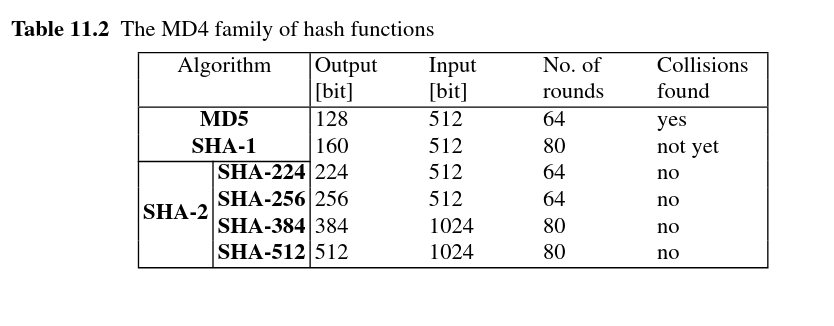
\includegraphics[scale=0.4]{md4table.png}
\end{figure}
This powerful algorithm had basically 4 design goals when it was presented:
\begin{enumerate}
    \item \textbf{Security}: it should be computationally infeasible to find  two messages MI and M2 that have the same message digest. Here we define a task to be “computationally infeasible” if it requires more than $2^64$ operations. 
    \item \textbf{Speed}: the algorithm should be as fast as possible. Here we are interested  in speed in software. In particular, we are interested in algorithms that are fast on 32-bit architectures, since that is becoming the dominant standard processor archi- tecture.  Thus, the algorithm should  be based on a simple set of primitive operations on 32-bit  words.
    \item \textbf{Simplicity and Compactness}: the algorithm should be simple to describe and simple to program,  without  requiring large programs or sub- stitution tables.
    \item \textbf{Favor little-endian architectures}: Some processor architectures (such as the Intel 8Oxxx line) are  “little endian”: they store the least- significant byte of a  word  in the low-address byte position. Others are “big-endian”: the most-significant byte of a word goes in the low- address byte position. This distinction is significant  when treating a message as a sequence of 32-bit  words,  since one architecture or the other will have to byte-reverse each word before  processing.
\end{enumerate}
The following algorithm description is taken directly from the paper in which Rivest presented MD4.
\newpage \underline{\textbf{MD4 Algorithm description}}
\newline\newline  \underline{Recall}: a work is a 32-bit quantity, while a byte is an 8-bit quantity. Therefore A sequence of bits  can be interpreted in a  natural manner as a  sequence of bytes, where each consecutive group of 8 bits is interpreted as a byte with the high-order (most significant) bit of each byte listed first. Similarly, a sequence of bytes  can be interpreted as a sequence of 32-bit words,  where  each consecutive group of 4 bytes is  interpreted as a word with the low-order (least significant) byte given first. 
\begin{figure} [H]
    \centering
    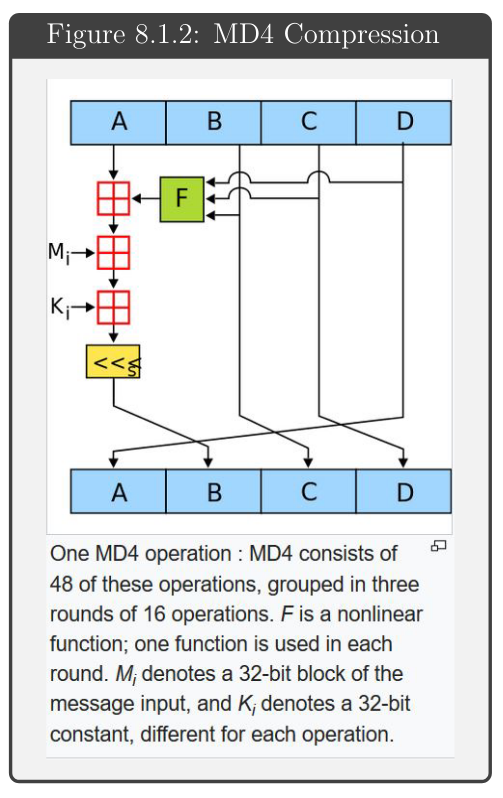
\includegraphics[scale=0.3]{md4figure.png}
\end{figure}
We begin by supposing that we have a b-bit message as input, and that we wish to find its message digest. Here b is an  arbitrary non negative  integer; b may be zero, it doesn't have to be a multiple of 8, and it may  be arbitrarily large. We imagine the bits of the message written down as $m_0m_1m_2...m_{b-1}$.
The following five steps are performed to compute the message digest of the message. 
\begin{enumerate}
    \item \textbf{Append padding bits:} The message is padded (extended) so that its length  (in bits) is congruent to 448, modulo 512. That is, the message is extended so that it is just 64 bits shy of being a  multiple of 512 bits long (simply because $448=64(mod512)$. Padding is  always performed, even if  the length of the message is  already congruent to 448, modulo 512 (in which case 512 bits of padding are added). Padding is performed as follows: a single “1” bit is appended to the message, and then enough zero bits are appended so that the length in bits of the padded message becomes congruent to 448, modulo 512. (This padding operation is invertible, SO that different inputs yield  different outputs-this would not  be true if we merely padded with 0’s.)
    \item \textbf{Append  length:} A 64-bit representation of b (the length of the message  before the padding  bits were added) is appended to the result of the previous step. These bits are appended as two 32-bit  words and appended low-order word first in accordance with the previous conventions. In the unlikely event that b is greater than $2^64$, then only the low-order 64 bits of b are used. At this point the resulting message (after padding  with bits  and  with b) has a length that is  an exact  multiple of 512 bits. Equivalently, this message has a length that is an exact  multiple of 16 (32-bit) words.  Let $M[0.. . N - 1]$ denote the words of the resulting message, where N is  a multiple of 16.
    \item \textbf{Initialize MD buffer:} A 4-word buffer (A, B, C, D) is used to compute the message digest.  Here each of A, B, C, D is a  32-bit register.  These  registers are initialized to some arbitrary values (in hexadecimal, low-order bytes first).
    \item \textbf{Process message in 16-word blocks:} We first  define three auxiliary functions that each take as input three 32-bit words and produce as output one 32-bit word. 
    \begin{itemize}
        \item $f(X,Y,Z)=XY \vee (\neg X)Z$
        \item $g(X,Y,Z)=XY \vee XZ \vee YZ$
        \item $h(X,Y,Z)=X \xor Y \xor Z$
    \end{itemize}
    In each bit position f acts as a conditional: if x then y else z. In each bit position g acts as a  majority function: if at least  two of x,y, z are one, then g has a one in that position. The function h is  the bit-wise xor or parity function.
    
    Optional: here's the loop implementation of the algorithm:
    \newline MD4 utilizes  two “magic constants”  in rounds  two and three. The round two constant is $\sqrt{2}$ (which in hex is 5A827999) and the round 3 constant is $\sqrt{3}$ (which in hex is 6ED9EBA1). These are basically the initialization vectors of the algorithm (Exercise 8.1.3).
    \item \textbf{Output:} The message digest  produced as output is A, B, C, D. That is, we begin with the low-order byte of A, and  end with the high-order byte of D. This completes the description of MD4.
\end{enumerate}
\begin{figure} [H]
    \centering
    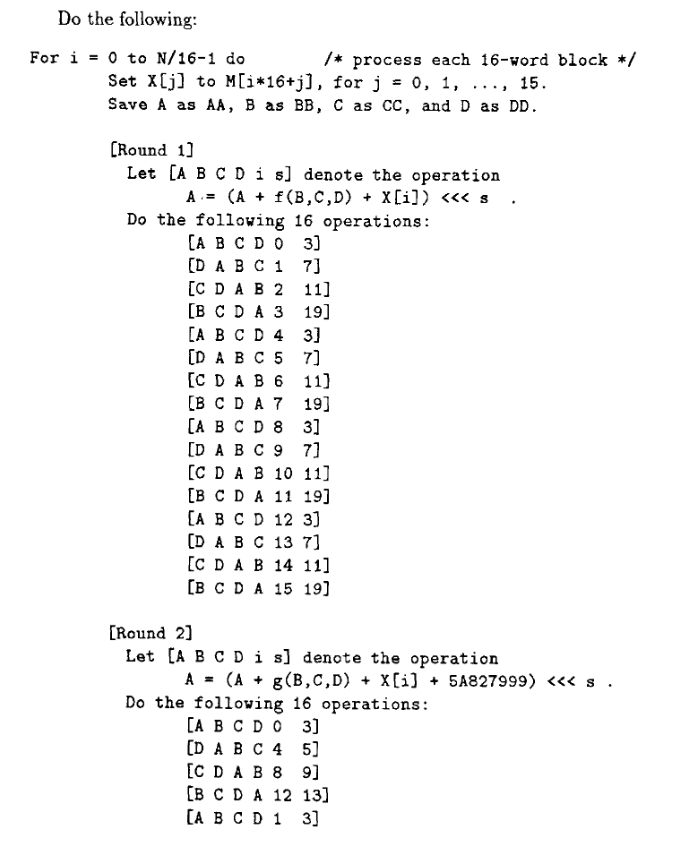
\includegraphics[scale=0.4]{md4loop.png}
\end{figure}
\begin{figure} [H]
    \centering
    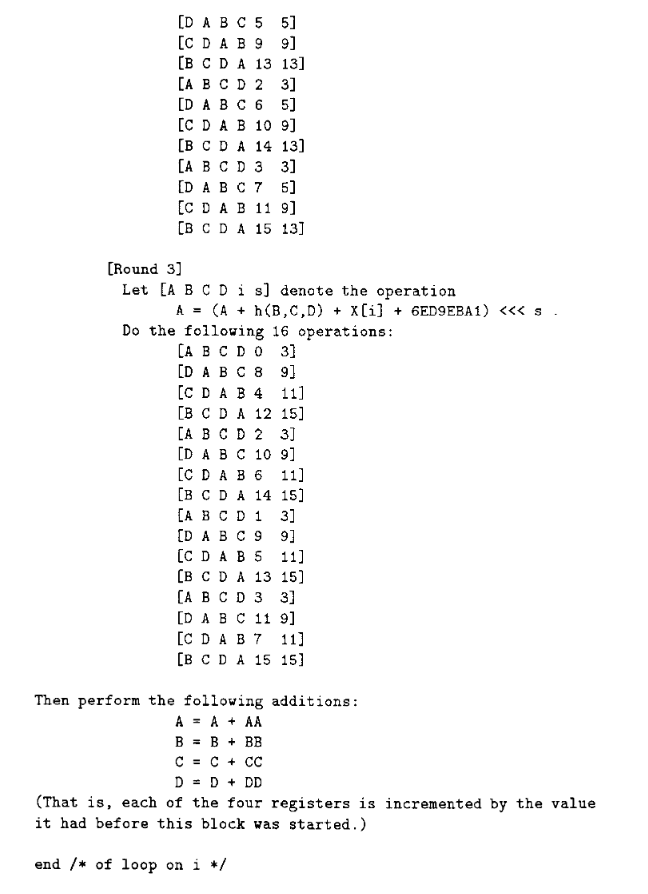
\includegraphics[scale=0.4]{md4loop2.png}
\end{figure}

\begin{figure} [H]
    \centering
    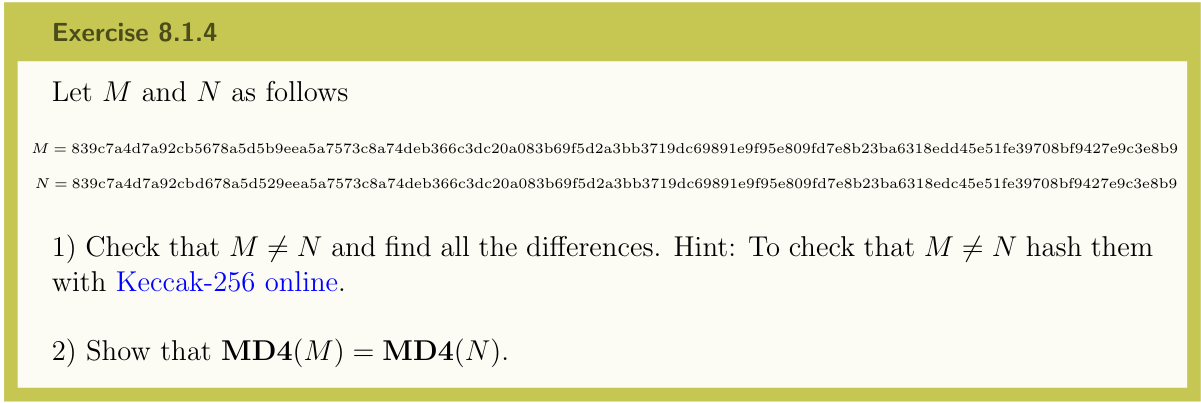
\includegraphics[scale=0.3]{ex8.1.4.png}
\end{figure}
\newline\newline\textcolor{red}{Solution}
\newline This is basically an example of collision attack, in which we have different data blocks that have the same hash function, namely MD4(M)=MD4(N).
\begin{figure} [H]
    \centering
    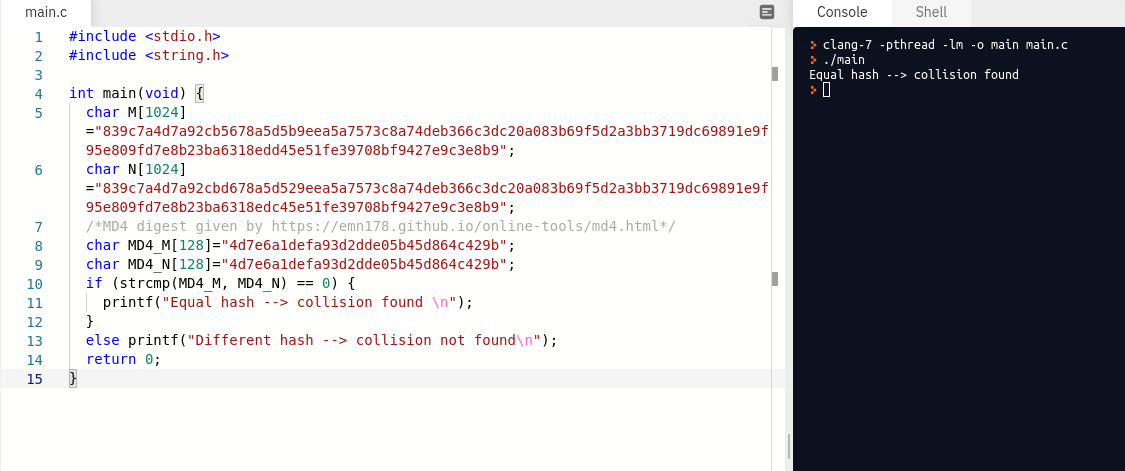
\includegraphics[scale=0.3]{sol.png}
\end{figure}
Remind: the collision attack relies on the birthday paradox.
\subsection{SHA-1}
The Secure Hash Algorithm (SHA-1) is the most widely used message digest function of the MD4 family. Even though new attacks have been proposed against the algorithm, it is very instructive to look at its details because the stronger versionsin the SHA-2 family show a very similar internal structure. SHA-1 is based on a Merkle–Damg̊ard constructio .An  interesting  interpretation  of  the  SHA-1  algorithm  is  that  the  compression function works like a block cipher, where the input is the previous hash value $H_{i−1}$ and the key is formed by the message block $x_i$ .As we will see below, the actual rounds of SHA-1 are in fact quite similar to a Feistel block cipher. SHA-1 produces a 160-bit output of a message with a maximum length of $2^64$ bit.Before the hash computation, the algorithm has to preprocess the message. During the actual computation, the compression function processes the message in 512-bit chunks. The compression function consists of 80 rounds which are divided into four stages of 20 rounds each.
\begin{figure} [H]
    \centering
    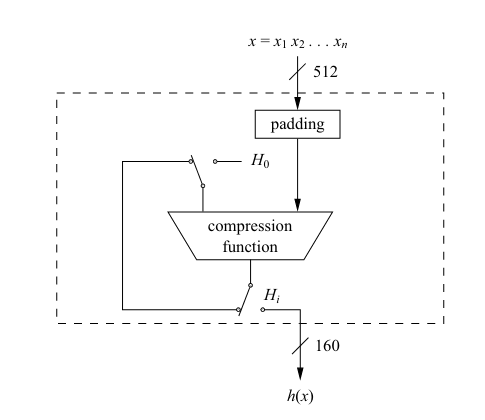
\includegraphics[scale=0.4]{sha-1diagram.png}
    \caption{High-level diagram of SHA-1}
\end{figure}
Basically the algorithm is divided in two phases:
\begin{enumerate}
    \item \textbf{Preprocessing:} Before the actual hash computation, the message $x$ has to be padded to fit a size of a multiple of 512 bit. For the internal processing, the padded message must then be divided into blocks. Also, the initial value $H_0$ is set to a predefined constant.
    \begin{itemize}
        \item \textbf{Padding}: Assume that we have a message $x$ with a length of $l$ bit. To obtain an overall message size of a multiple of 512 bits, we append a single “1” followed by $k$ zero bits and the binary 64-bit representation of $l$. Consequently, the number of required zeros $k$ is given by:
        \begin{equation*}
            k \equiv 512-64-1-l = 448-(l+1) mod512
        \end{equation*}
        \begin{figure} [H]
            \centering
            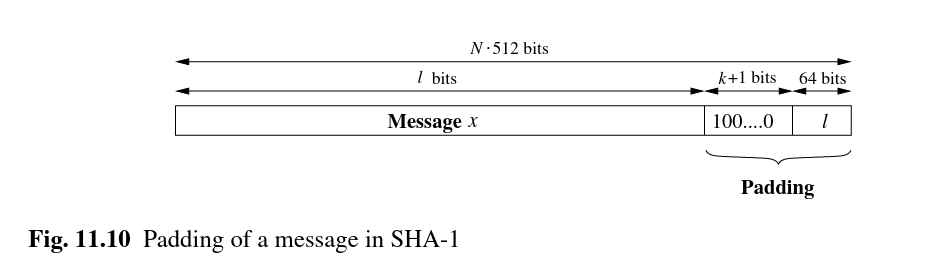
\includegraphics[scale=0.3]{paddingsha-1.png}
        \end{figure}
        Example: Given is the message “abc” consisting of three 8-bit ASCII characters with a total length of$l=24$ bits:
        \begin{figure} [H]
            \centering
            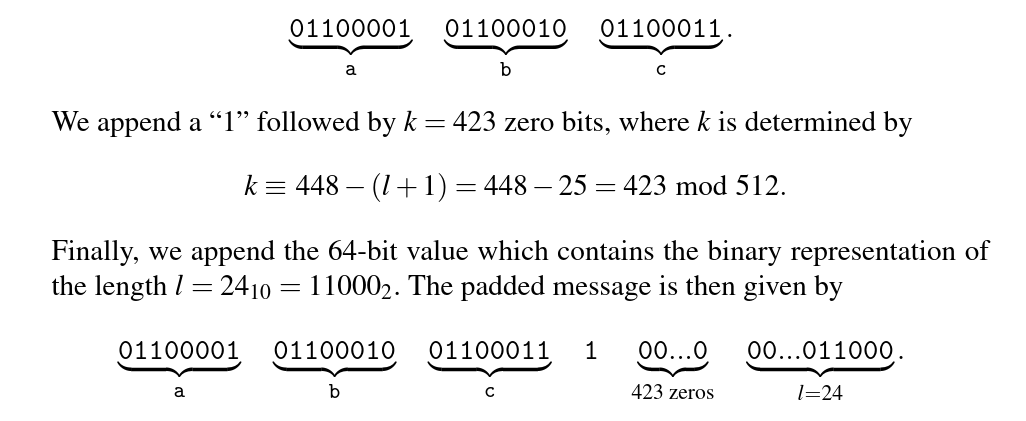
\includegraphics[scale=0.3]{examplesha-1.png}
        \end{figure}
        \item \textbf{Dividing the padded message:} Prior  to  applying  the  compression  function,  we need to divide the message into 512-bit blocks $x_1,x_2, ... ,x_n$. Each 512-bit block can be subdivided into 16 words of size of 32 bits. For instance, the i-th block of the message $x$ is split into:
        \begin{equation*}
            x_i = (x_i^{(0)}x_i^{(1)}...x_i^{(15)})
        \end{equation*}
        where $x_i?{(k)}$ are words of size of 32 bits.
        \item \textbf{Initial value $H_0$:} A 160-bit buffer is used to hold the initial hash value for the first iteration. The five 32-bit words are fixed and given in hexadecimal notation as:
        \begin{figure}  [H]
            \centering
            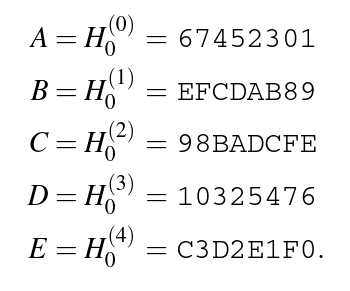
\includegraphics[scale=0.4]{sha-1words.png}
        \end{figure}
    \end{itemize}
    \item \textbf{Hash computation:} Each message block $x_i$ is processed in four stages with 20 rounds each. The algorithm uses:
    \begin{itemize}
        \item a message schedule which computes a 32-bit word $W_0,W_1, ...,W_79$ for each of the 80 rounds. The words $W_j$ are derived from the 512-bit message block as follows:
        \begin{figure} [H]
            \centering
            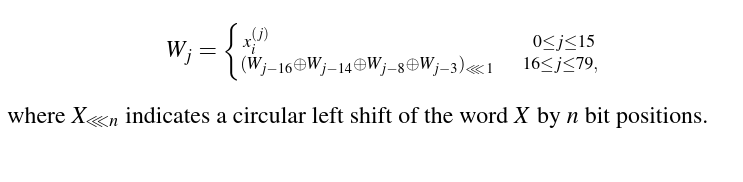
\includegraphics[scale=0.4]{sha-1wordswj.png}
        \end{figure}
        \item five working registers of size of 32 bits A,B,C,D,E
        \item a hash value $H_i$ consisting of five 32-bit words $H_i^{(0)},H_i^{(1)},H_i^{(2)},H_i^{(3)},H_i^{(4)}$. In the beginning, the hash value holds the initial value $H_0$, which is replaced by a new hash value after the processing of each single message block. The final hash value $H_n$ is equal to the output $h(x)$ of SHA-1.
    \end{itemize}
    \begin{figure} [H]
        \centering
        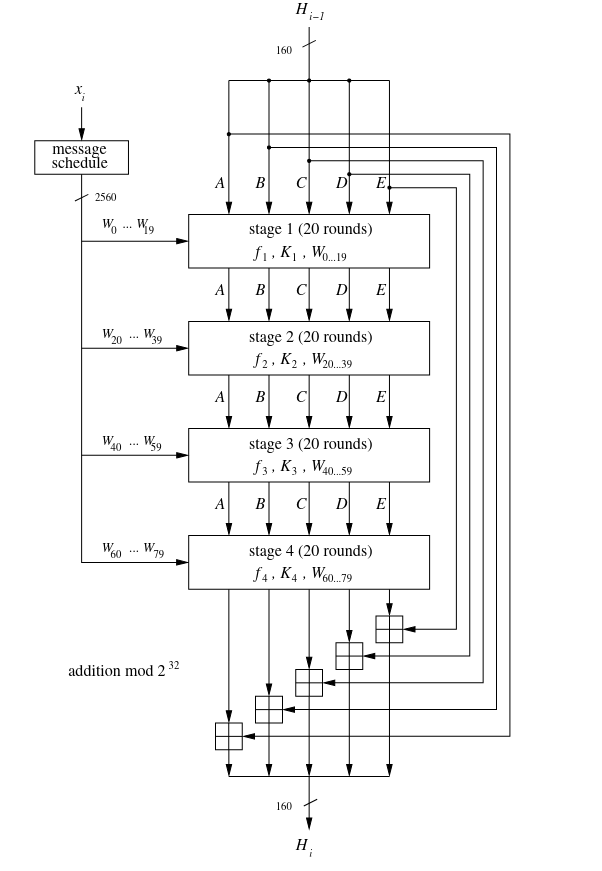
\includegraphics[scale=0.45]{sha-1scheme.png}
    \end{figure}
    The four SHA-1 stages have a similar structure but use different internal functions $f_t$ and constants $K_t$ ,where $1 \leq t \leq 4$. Each stage is composed of 20 rounds, where parts of the message block are processed by the function $f_t$ together with some stage-dependent constant $K_t$. The output after 80 rounds is added to the input value $H_{i-1} mod232$ in word-wise fashion.
    \newline\newline The operation within round j in stage t is given by
    \begin{equation*}
        A,B,C,D,E=(E+f_t(B,C,D)+(A)_{\lll 5} +W_j+ K_t),A,(B)_{\lll 30},C,D
    \end{equation*}
    \begin{figure} [H]
        \centering
        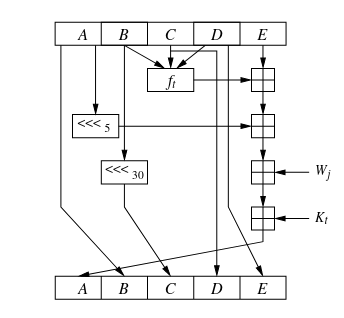
\includegraphics[scale=0.4]{sha-1roundj.png}
        \caption{Round j in stage tof SHA-1. It has some resemblance to the round ofa Feistel network. Feistel networks are generally characterized by the fact the first part of the input is copied directly to the output. The second part of the input is encrypted using the first part, where the first part is sent through some function}
    \end{figure}
    \newline The internal functions $f_t$ and constants $K_t$ change depending on the stage according to the table shown below, i.e., every 20 rounds a new function and a new constant are being used. The function only uses bitwise Boolean operations, namely logical AND, OR, NOT and XOR.  In the  SHA-1  round,  the  inputs A,B,C and D arepassed to the output with no change (A,C,D), or only minimal change (rotation of B). However, the input word E is “encrypted” by adding values derived from the other four input words. The message-derived value $W_i$ and the round constant play the role of subkeys.
    \begin{figure} [H]
        \centering
        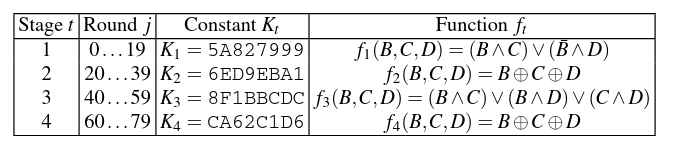
\includegraphics[scale=0.45]{sha-1table.png}
        \caption{Round functions and round constants for the SHA rounds}
    \end{figure}
\end{enumerate}

\begin{figure} [H]
    \centering
    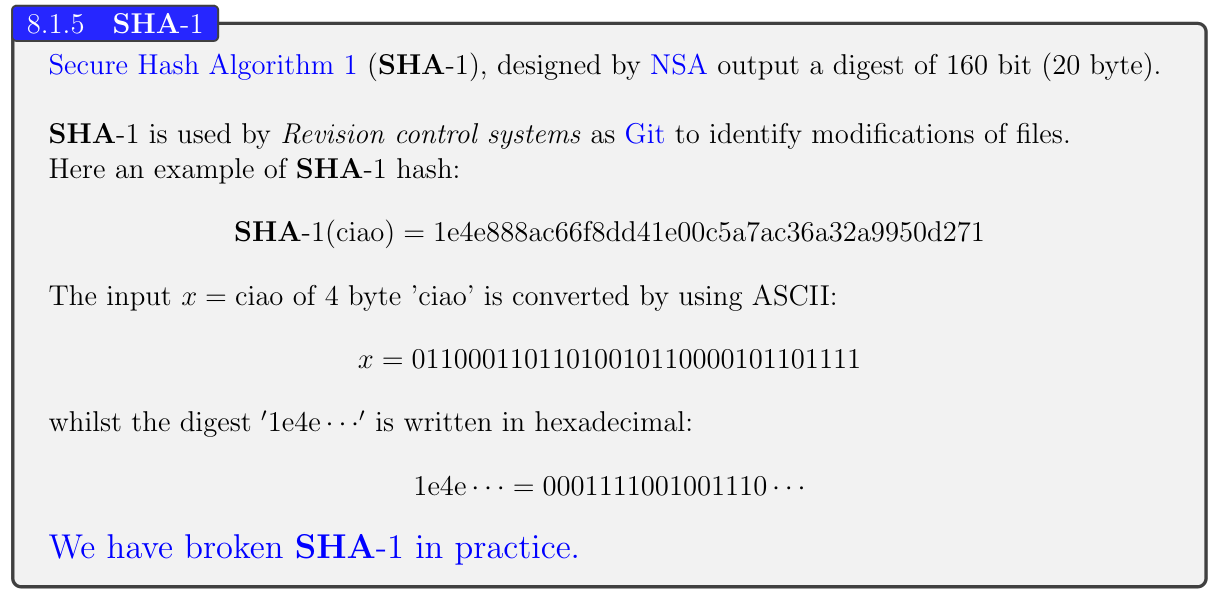
\includegraphics[scale=0.3]{example2sha-1.png}
    \caption{Here we have a practical example of SHA-1.}
\end{figure}
\subsection{The SHA-2 Family}
SHA-2, the successor to SHA-1, was designed by the NSA and
standardized by NIST. SHA-2 is a family of four hash functions: SHA-
224, SHA-256, SHA-384, and SHA-512, of which SHA-256 and SHA-
512 are the two main algorithms. The three-digit numbers represent the
bit lengths of each hash. This algorithm is meant to provide 128 bits of security against collision attacks.

\subsubsection{SHA-256}
\newline SHA-256 operates in the manner of MD4, MD5 and SHA-1. The message to be hashed is first:
\begin{enumerate}
    \item padded with its length in such a way that the result is a multiple of 512 bits long, and then
    \item parsed into 512-bit message blocks $M^{(1)}, M^{(2)}, ..., M^{(N)}$.
\end{enumerate}
The message blocks are processed one at a time: beginning with a fixed initial hash value $H^{(0)}$, sequentially compute
\begin{equation*}
    H^{(i)}=H^{(i-1)} + C_{M^{(i)}}(H^{(i-1)}
\end{equation*}
Where $C$ is the SHA-256 \textit{compression function} and + means word-wise $mod2^32$ addition. $H^{(N)}$ is the hash of $M$.
\begin{figure} [H]
    \centering
    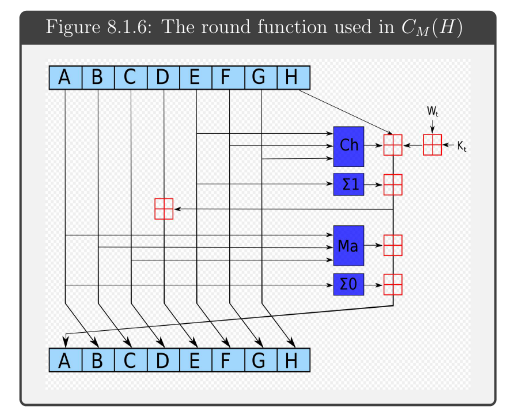
\includegraphics[scale=0.4]{sha-2.png}
    \caption{A, B, C, D, E, F, G, H are words of 32 bits. Each 512 block $M^{(0)}$ is regarded as a key of a block-cipher Enc which cipher plaintext is $H^{(i-1)}$. There are 64 rounds, while $K_t$ are fixed constants (depending on the round) and $W_t$ is part of the key-schedule of Enc.}
\end{figure}
The SHA-256 compression function operates on a 512-bit message block and a 256 bit intermediate hash value. It is essentially a 256-bit block cipher algorithm which encrypts the intermediate hash value using the message block as a key. Hence there are two main components to describe the SHA-256 compression function and the SHA-256 message schedule. 
\section{Keccak and the SHA-3 Family}
\begin{figure} [H]
    \centering
    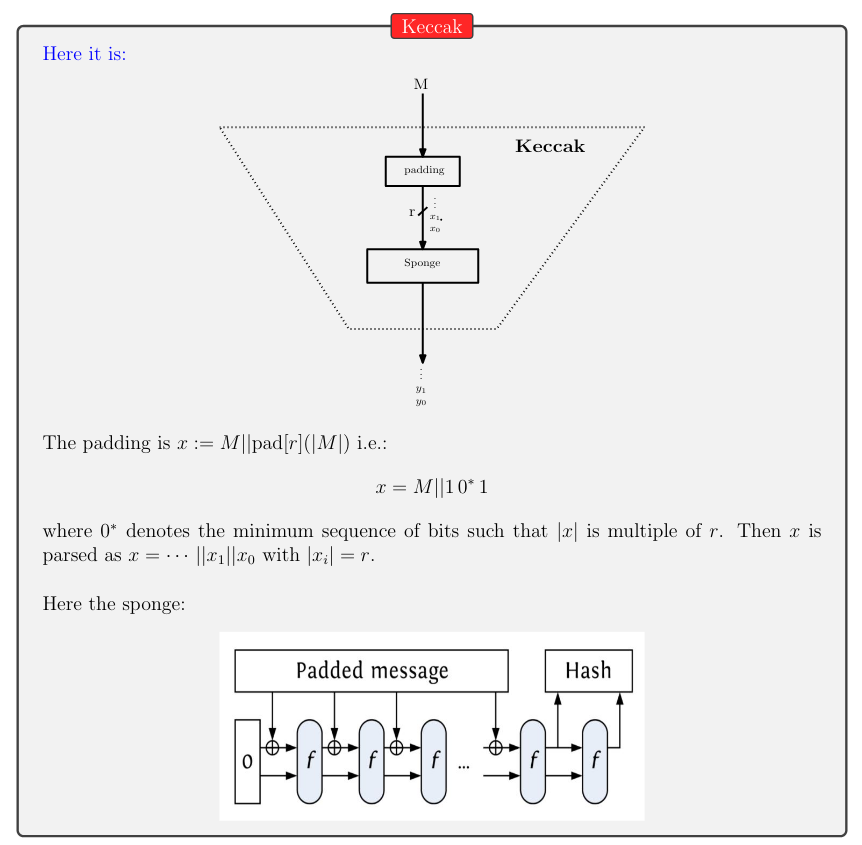
\includegraphics[scale=0.4]{sha-3keccak.png}
\end{figure}
Keccak’s core algorithm is a permutation of a 1600-bit state that ingests
blocks of 1152, 1088, 832, or 576 bits, producing hash values of 224, 256,
384, or 512 bits, respectively—the same four lengths produced by SHA-2 hash functions. But unlike SHA-2, SHA-3 uses a single core algorithm rather than two algorithms for all four hash lengths.
Another reason is that Keccak is more than just a hash. The SHA-3
standard document FIPS 202 defines four hashes (SHA3-224, SHA3-
256, SHA3-384, and SHA3-512) and two algorithms called SHAKE128
and SHAKE256. These two algorithms are extendable-output functions (XOFs), or hash functions that can produce hashes of variable length, even very
long ones. The numbers 128 and 256 represent the security level of each algorithm. If you want to see a C implementation of the Keccak core algorithm, go to \url{https://github.com/mjosaarinen/tiny_sha3/blob/master/sha3.c}.

\end{document}

